\renewcommand{\x}{\mathbf{x}}
\renewcommand{\v}{\mathbf{v}}
\renewcommand{\w}{\mathbf{w}}
\newcommand{\B}{\mathcal{B}}
\newcommand{\egsum}{c_1\mathbf{e}_1+\c_2\mathbf{e}_2+\cdots+c_n\mathbf{e}_n}
\newcommand{\egmatrix}{\begin{pmatrix}
    |& \ & | \\
    \mathbf{a}_1& \cdots& \mathbf{a}_n \\
    |& \ & | \\
\end{pmatrix}}
\newcommand{\egbasis}{\{\mathbf{b}_1,\mathbf{b}_2,\cdots,\mathbf{b}_n\}}

Here's a short introduction about what this chapter will be about. We have many kinds of vector spaces, and the computation is quite complex. Therefore, we want to come up with a more general way so that we can compute different linear transformations in the same form. This universal language of linear transformation is called matrix. To develop this chapter, we follow the following logic:\\

1. Show that a matrix stands for a linear transformation in Euclidean space.\\

2. Converting any linear transformation into a matrix. We need to study some of the properties of linear transformations before that.








\section{Matrix}
We now introduce the concept of matrix. In different context, matrix represents different kinds of things. In computer science, people sometimes regard 2-d array as matrix. But in the context of linear algebra, a matrix is usually a linear transformation on Euclidean space.\\

We consider the space $\mathbf{R}^n$, it's a n-dimensional vector space, the most natural way of finding a basis is $$\mathcal{E} =
\{\mathbf{e}_1,\mathbf{e}_2,\cdots,\mathbf{e}_n\}:=\{
\begin{pmatrix}
    1\\
    0\\
    \vdots\\
    0
\end{pmatrix},\begin{pmatrix}
    0\\
    1\\
    \vdots\\
    0
\end{pmatrix},\cdots, \begin{pmatrix}
    0\\
    0\\
    \vdots\\
    1
\end{pmatrix}
\}$$
Therefore, when we want to describe a linear transformation, we only need to describe how each of the elements was mapped to.For a linear transformation $T$, we put all resulting vectors in a list of columns. For example:
$$T(\mathbf{e}_1) = \mathbf{a}_1,T(\mathbf{e}_2) = \mathbf{a}_2,\cdots,T(\mathbf{e}_2) = \mathbf{a}_n$$
The matrix of linear transformation is 
$$\egmatrix$$.
Since $$\begin{pmatrix}
    c_1\\c_2\\\vdots\\c_n
\end{pmatrix}
 = 
 c_1\mathbf{e}_1+c_2\mathbf{e}_2+\cdots+c_n\mathbf{e}_n$$
We have
$$T(\mathbf{v}) =c_1\mathbf{a}_1+c_2\mathbf{a}_2+\cdots+c_n\mathbf{a}_n $$

We usually denote the matrix with each columns as the ``sent'' vectors from the $\mathbf{e}_1 \cdots$ as the matrix of linear transformation of Euclidean space. For example, if\\
$$T(\mathbf{e}_1) = \begin{pmatrix}
    1\\
    2
\end{pmatrix},T(\mathbf{e}_2) = \begin{pmatrix}
    2\\
    3
\end{pmatrix}$$we can say $$A = \begin{pmatrix}
    1\ 2\\
    2\ 3 
\end{pmatrix}$$
is the matrix of the linear transformation. Also:\\
$$T(\begin{pmatrix}
    1\\2
\end{pmatrix}) = A\begin{pmatrix}
    1\\2
\end{pmatrix} = 1\begin{pmatrix}
    1\\
    2
\end{pmatrix}+2\begin{pmatrix}
    2\\
    3
\end{pmatrix}$$

\section{Matrix multiplication}
Intuitively, a combination of linear transformation is still a linear transformation. That means we can still represent combination of linear transformation with another matrix. Now lets figure out the relation between them. Then let's consider:

$$A = \egmatrix\ B = \begin{pmatrix}
    |& \ & | \\
    \mathbf{b}_1& \cdots& \mathbf{b}_n \\
    |& \ & | \\
\end{pmatrix}$$
The i-th column of the combination of the two LT (Later I will use LT as linear transformation) is given by $AB\mathbf{e}_i = A\mathbf{b}_i$. Therefore, we express $$AB = \begin{pmatrix}
    |& \ & | \\
    A\mathbf{b}_1& \cdots& A\mathbf{b}_n \\
    |& \ & | \\
\end{pmatrix}$$
That makes a lot of sense! And if we consider an vector as a LT from a real number to vector, the computation of matrix is compatible with matrix multiplication! (Which is good)

\subsection{Nonlinearity of neural network}

There's some fun fact about deep learning. In deep learning, there's a very important structure called MLP (multi-layers preceptor). If we consider the easiest case in deep learning, maybe recognizing numbers? What we actually do is to map an image into it's label, which can be both considered to be Euclidean space. \\

To further elaborate this point, consider an image with size $20\times20$. We can in fact consider it as an vector in $\mathbf{R}^{400}$, since it has $400$ blocks. And we want to find a mapping from $\mathbf{R}^{400}$ to $\mathbf{R}^{10}$, which is the range of all the numbers (In machine learning, we call these labels). The idealistic situation is, we input an image(vector) and output a vector say $\mathbf{e}_3$, which correspond to 3.\\

\begin{figure}[h]
    \centering
    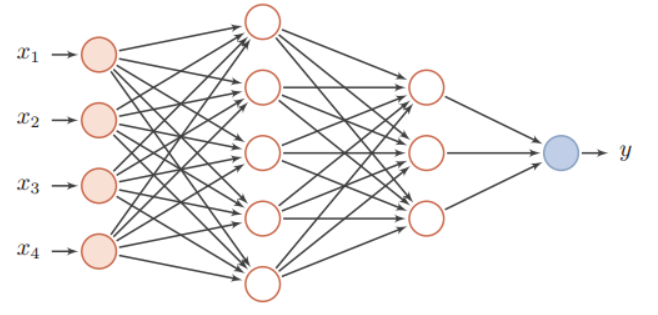
\includegraphics[width=0.5\textwidth]{Chapters/nn.PNG}
    \caption{This is an example}
    \label{fig:example}
\end{figure}

The most natural way people would come up is to use LT to simulate this mapping, because computer would really love to compute LT (easier). They later want to increase the number of parameters (the number of matrices), so that the performance of the network might be better. However, if we just arbitrarily put many matrices together, nothing will work. Since the combination of LT is still LT, which can be represented by a single matrix.

To deal with that, people usually add an element-wise non-linear function. Therefore, the combination of all matrices will not become a simple matrix!

I think I haven't explain this part clear enough, if you are interested, maybe you can check out the video of 3Blue1Brown. He has a wonderful video talking about this concept.  

\section{Injective, Surjective and Bijective}
In this part, we will deal with some properties of LT, which is essential when we want to convert an arbitrary LT into a matrix. 
\begin{definition}
    Consider a LT $T$ from $V$ to $W$.\\
    A LT is injective (one to one) if $T(\v) = T(\w)$ will imply $\v = \w$\\
    A LT is surjective (onto) if $\forall \w \in W\ \exists \v \in V$ with $T(\v) = \w$\\
    A LT is bijective if it's both injective and surjective. 
\end{definition}
Note that sometimes we call a bijective function an isomophism. These definitions might be a little weird to you, let's explain their meanings. These properties usually serve for the existence of inverse, another function $T^{-1}$ with $TT^{-1} = I$, where $I$ is the LT map every element to itself. We will get back to it later.\\

If you have some background information in calculus, you would know that $e^x$ is the inverse of $log(x)$. we have $e^{log(x)} = log(e^{x}) = x$. In the context LT, we also want something similar. But the first important thing is that we have to make sure the co-domain and domain have one to one relation. If $f(1) = 2\ f(3) = 2$, what is $f^{-1}(2)$ supposed to be? We cannot expect a funcion will output two values at the same time. Therefore, injective is the first necessary condition of existence of inverse.\\

Now if a function is injective, can we conclude that it's invertible? No! We also need to pay attention to the value that nothing would map to. They are like the single guys from a party. If you want to find a invertible matrix, you have to find each of them a partner, that is exactly the expression of surjective!\\

Hence we can sum up.
\begin{theorem}
    If LT is bijective, then dim $V$ = dim $W$. Also, $\exists T^{-1}$, with $TT^{-1} = I$, $T^{-1}T = I$. 
\end{theorem}
Note that even $TT^{-1}$ and $T^{-1}T$ will both give an $I$, but they are actually different. Because they are defined in different spaces. One map $W$ to $W$, and other map $V$ to $V$. The proof is omitted there because I'm lazy to type. But I think the above explaination will be a good source for understand. 
\begin{note}
    We also have two equivalent way to express injective and surjective. \\
    If $T$ is injective, Ker$T$ := \{$\v$: $T(\v) = \mathbf{0}$\} = \{$\mathbf{0})$\}.(:= means defined as)\\
    If $T$ is surjective, $T(V):=\{\w: \exists \v$ with $T(\v) = w\}$ = $W$\\
    If T is injective, we can show that dim$T(V) = $dim$W$, combining this and $T$ is surjective, we can show the dimension of two vector space are the same.
\end{note}
Sometimes if we want to show that two set are equal, we can show that $A \subset B$ and $B\subset A$. Try this to show If $T$ is surjective, $T(V):=\{\w: \exists \v$ with $T(\v) = w\}$ = $W$.

We also should mention the inverse of combiniation of invertible LT.
\begin{theorem}
    If LT $S$ and $T$ are both invertible, then their combination is also invertible, with $(ST)^{-1} = T^{-1}S^{-1}$
\end{theorem}
You can simply multiply the inverse with the original LT to show it's indeed the inverse.


\section{Use Matrix to represent a linear transformation}
It's such a long section name, but the following indeed will give us a very beautiful result, or even the most important result of linear algebra. That is, every LT can be represented using a matrix.\\

We know that every finitely dimensional LT will map from a vector space to another. A vector space has an integer dimension. Then we have the following map.\\
\begin{theorem}
    If we have a vector space $V$ whose dimension is $n$ and a basis $\mathcal{B}$ $\egbasis$, then we have the following mapping from $V$ to $\mathbf{R}^n$:
    $$\psi_{\mathcal{B}}(\v) = c_1\mathbf{b}_1+c_2\mathbf{b}_2+\cdots+c_n \mathbf{b}_n = \begin{pmatrix}
        c_1\\c_2\\ \vdots\\c_n
    \end{pmatrix}$$
\end{theorem}
This is a direct consequence of Theorem 1.9, which is decomposition theorem. By checking the property, we know that this function is bijective. (Leave as an exercise for readers) Therefore, without doubt, it's an invertible function! \\

Then let's consider this, if we first map $\v$ to another vector in $\mathbf{R}^n$, passing through a matrix, and map it from $\mathbf{R}^m$ back to $V$ (dimension might have changed here), we are then able to express the general LT with matrix. In other word $$T = \psi^{-1}_{\mathcal{B}_2}A\psi_{\mathcal{B}_1}$$
Very Importantly! We usually consider combination of functions from right to left (even though we might read from right to left).\\

Then the matrix is given by
$$[T]_{\mathcal{B}_2\mathcal{B}_1} = A = \psi_{\mathcal{B}_2}T\psi_{\mathcal{B}_1}^{-1}$$ 
$[T]_{\mathcal{B}_2\mathcal{B}_1}$ is considered to be: the matrix representing linear transformation $T$ from the vector space $V$ represented by basis $\mathcal{B}_1$, to vector space $W$ represented by basis $\mathcal{B}_2$, which itself would be a matrix mapping from $\mathbf{R}^n$ to $\mathbf{R}^m$. Let's see an example~
\subsection{Vandermonde Matrix}

There's an very interesting property of polynomials, that any polynomial of degree $n$ can be represented by $n+1$ points. On the other hand, if we know the $n+1$ points and the cooresponding coordinate, we can determine the polynomial.\\

It becomes trivial to consider the following map called evaluation map. 
\begin{definition}
    Given n+1 distinct points $t_0,t_1,\cdots,t_n$ and a polynomial $p(x)$, we have the following map:
    $$T(p(t)) = \begin{pmatrix}
        p(t_0)\\p(t_1)\\ \vdots\\p(t_n)
    \end{pmatrix}$$

\end{definition}

We know that a polynomial can be represented by a list of coefficients. For example, $3x^2+2x+1$ can be represented by $(1,2,3)$. Then we have the following coordinate mapping :
$$\psi_{\{1,t,t^2,\cdots,t^n\}}(x_0+x_1t+\cdots+x_nt^n) = \begin{pmatrix}
    x_0\\x_1\\ \vdots \\x_n
    \end{pmatrix}$$

Then we want to express the evaluation map with a matrix. We follow the following logic:
$$[T]_{\mathcal{B}_2\mathcal{B}_1}(\mathbf{e}_i) = A = \psi_{\mathcal{B}_2}T\psi_{\mathcal{B}_1}^{-1}(\mathbf{e}_i) = \psi_{\mathcal{B}_2}T(t^{i}) = \psi_{\mathcal{B}_2}\begin{pmatrix}
    t_0^i\\t_1^i \\ \vdots \\t_n^i
\end{pmatrix} = \begin{pmatrix}
    t_0^i\\t_1^i \\ \vdots \\t_n^i
\end{pmatrix}$$
Note that the $T$ will map from $P_n[t]$ to $\mathbf{R}^{n+1}$. Here, $\mathcal{B}_1$ is the standard basis of polynomial, and $\mathcal{B}_2$ is just standard basis of Euclidean space. The last step is basicly an identity map. This will indeed give us the Vandermonde matrix.\\
$$
\begin{pmatrix}
    1 & t_0 & t_0^2 & \cdots & t_0^n\\
    1 & t_1 & t_1^2 & \cdots & t_1^n\\
    \vdots & \vdots & \vdots & \ddots & \vdots\\
    1 & t_n & t_n^2 & \cdots & t_n^n
\end{pmatrix}
$$
Please! Feel free to test whether this will give you the desired results. Also, the matrix is invertible, if we want to solve the inverse matrix, we should consider Lagrange interpolate. Relevant information can be found in wikipedia.

\section{Change of basis and Similar matrix}

In last chapter, when we use a matrix to represent a LT, we have an important move, we select a basis from the original $V$ and build a bijective coordinate map. It becomes natural for us to consider, if we change to another basis, what will actually happen? \\

This discussion lead to the research on ``change of basis''. For simplicity, we usually discuss the LT whose $V$ and $W$ are of the same dimension. Then we have
$$[T]_{\B_1 \B_1} = \psi_{\B_1}T\psi_{\B_1}^{-1}\ $$
$$[T]_{\B_2 \B_2} = \psi_{\B_2}T\psi_{\B_2}^{-1}\ $$
Therefore
$$[T]_{\B_2 \B_2} = \psi_{\B_2}\psi_{\B_1}^{-1}[T]_{\B_1 \B_1}\psi_{\B_1}\psi_{\B_2}^{-1}$$
We can then try to understand the meaning of $\psi_{\B_1}\psi_{\B_2}^{-1}$, this function will receive a vector from $\mathbf{R}^n$ and convert it into $V$, then coordinate map it to $\mathbf{R}^n$ again. Obviously, it's a LT on Euclidean space. Then it can be represented as a matrix, we denote it as $P_{\B_1 \B_2}$.\\

The i-th column of $P_{\B_1 \B_2}$ will be the obtained vector from $\mathbf{e}_i$, then $\psi_{\B_1}\psi_{\B_2}^{-1}(\mathbf{e}_i) = \psi_{\B_1}(\mathbf{b_{2i}}):=[\mathbf{b_{2i}}]_{\B_1}$ 
Therefore
$$P_{\B_1 \B_2} = \begin{pmatrix}
    |& \ & | \\
    [\mathbf{b_{21}}]_{\B_1}& \cdots& [\mathbf{b_{2n}}]_{\B_1} \\
    |& \ & | \\
\end{pmatrix}$$
The notation here might be a little confusing and different textbook might use different notation. In this case, $\mathbf{b_{2i}}$ would mean the i-th vector in the basis $\B_2$.
And $[\mathbf{b_{2i}}]_{\B_1}$ would mean the coordinate vector of $\mathbf{b_{2i}}$ in terms of basis $\B_1$.\\

We are also aware of the fact that $\psi_{\B_2}\psi_{\B_1}^{-1}=(\psi_{\B_1}\psi_{\B_2}^{-1})^{-1}$. To sum up, we have 
$$[T]_{\B_2 \B_2} = P_{\B_1 \B_2}^{-1}[T]_{\B_1 \B_1}P_{\B_1 \B_2} = P_{\B_2 \B_1}[T]_{\B_1 \B_1}P_{\B_2 \B_1}^{-1}$$
Basicly, we obtain the matrix in terms of $\B_2$, we first change vector to basis of $\B_1$, operate the obtained vector and convert it into $\B_2$.\\

Sometimes, it's a little troublesome to find $P_{\B_1 \B_2}$. A practical experience is to use standard basis of $\mathbf{R}^n$, because $P_{ \varepsilon \B} = \begin{pmatrix}
    |& \ & | \\
    \mathbf{b}_1& \cdots& \mathbf{b}_n \\
    |& \ & | \\
\end{pmatrix}$, which is much easier to compute. Therefore 
$$P_{\B_1 \B_2} = P_{\varepsilon \B_1}^{-1}P_{\varepsilon \B_2} = \begin{pmatrix}
    |& \ & | \\
    \mathbf{b}_{11}& \cdots& \mathbf{b}_{1n} \\
    |& \ & | \\
\end{pmatrix}^{-1}\begin{pmatrix}
    |& \ & | \\
    \mathbf{b}_{21}& \cdots& \mathbf{b}_{2n} \\
    |& \ & | \\
\end{pmatrix}$$
\begin{eg}
    Consider the two basis:\\
    $$\B_1 = \{
        \begin{pmatrix}
            1\\1
        \end{pmatrix},
        \begin{pmatrix}
            1\\-1
        \end{pmatrix}\},
    \B_2 = \{
        \begin{pmatrix}
            1\\0
        \end{pmatrix},
        \begin{pmatrix}
            1\\1
        \end{pmatrix}\}$$\\
        Then $$P_{\varepsilon \B_1}=\begin{pmatrix}
            1 \ & 1\\1 \ & -1
        \end{pmatrix}, P_{\varepsilon \B_2}=\begin{pmatrix}
            1 \ & 1\\0 \ & 1
        \end{pmatrix}$$\\  

        $$P_{\B_1 \B_2} = \begin{pmatrix}
            1 \ & 1\\1 \ & -1
        \end{pmatrix}^{-1}\begin{pmatrix}
            1 \ & 1\\0 \ & 1
        \end{pmatrix}$$
\end{eg}

So far I haven't told you about how do we compute the inverse of a matrix. I will leave this kind of work to next chapter.

One thing that I should mention is the concept of similar matrix.
\begin{definition}
    Considering two matrix of the same size, if there exists an invertible matrix $P$, such that 
    $$B = PAP^{-1}$$ Then we say $A$ and $B$ are similar.
\end{definition}
In this case, we can consider the two matrix are representing the same LT, that's why we call it similar. Since they describe the same LT, any quantities defined on the LT are shared by the matrices. \\

Moreover, sometimes if we choose a ``nice'' basis, the matrix will look very nice, this is one of the key propose we will be working on. 

\section{Summary}
Let's do some summary. In this chapter, we first studied a special type of LT, which is LT in Euclidean space, and we represent that by a beautiful structure, matrix. Then by introducing some properties of LT (will be discussed later), we connect an arbitrary LT with matrix, then discussed different matrix to represent a LT and their relations. \\

In next chapter, we will solve some problems that we have left in this chapter.  Like how do we know the inverse of the matrix? Good luck!

